% Authors' response
\documentclass{scrartcl}
\usepackage[utf8]{inputenc}
\usepackage[english]{babel}
\usepackage{xcolor}
\usepackage{graphicx}
\usepackage{hyperref}
\usepackage{multirow}
\thispagestyle{empty}

\begin{document}
\section*{Authors' response}
To bg-2021-260-RC1 (05 Nov 2021):
We thank the anonymous referee \#1 for their comments.
We will address all \textbf{general comments} raised regarding the structure and readability of the manuscript in our next revision or resubmission. We consider to separate the manuscript in Introduction--Methods--Results--Conclusions and will improve on the "methods" Section to make our results more comprehensible. We will refine the language to reduce ambiguity and supplement our statements with appropriate citations where indicated by the referee.\\
As the manuscript will, hence, undergo major structural changes, we will not address all \textbf{specific / technical comments} in detail at this point. We will take all specific and technical comments which are still relevant into consideration.\\
In the following, we shall give a brief respond to all relevant issues.

\subsection*{General comments} 
\begin{itemize}
    
    \item {\color{blue} "the [...] study is highly speculative and not based on any experimental evidence [...]"} In the revision of our work, we will emphasize that the main objective of our work is to explore the possibilities of readily accessible data (i.e. long-term meteorological temperature observations, $\mathrm{CO_2}$ flux estimations from remote sensing) to provide alternatives to site-specific data that is needed to parameterize plant physiology in models such as the $\mathrm{DO_3SE}$ model used in our study.
    \item {\color{blue} "Many claims sound superficial [...], such as [...] the alleged deviation of the years 2018 and 2019 from the site's climatology [...]"} We strongly disagree with this statement. We assessed the particular years 2018 and 2019 by statistical means with respect to our derived climatologies. We acknowledge that we have not used common tools such as the \emph{p-value} (for a discussion see \href{https://doi.org/10.1080/00031305.2016.1154108}{statement of the American Statistical Association (2016)}).
    \item {\color{blue} "The manuscript is too long and the organization is confused  [...] no clear division between methodological section and results section"} We will address this in the next revision.

\end{itemize}

\subsection*{Specific comments} 
\begin{itemize}
    
\item {\color{blue}Lines 51-52. "and leads to a build-up of ozone and its precursors during winter." Are you sure? How can BVOC accumulate in the atmosphere if the vegetation is covered by snow? Please add some citations to support this claim. Much more credible is the following explanation based on stratospheric intrusions.}
We agree with the referee that a vegetation covered by snow would not release BVOCs to the atmosphere. We implicitly assume this. Therefore, we did not explicitly state that BVOCs are not among the ozone precursors that accumulate in the course of winter. We will rephrase the sentence accordingly: "[...] ozone and its non-biogenic precursors [...]"

\item {\color{blue}Line 63. "the time in which vegetation can accumulate ozone." 
It sounds very bad written this way: vegetation does not accumulate ozone because ozone it is not bioaccumulative. Did you mean the dose?}
Thank you for pointing this out. We will rephrase accordingly and refer instead the accumulated ozone dose.

\item {\color{blue}Line 77. "($\left<[\mathrm{O_3}]\right>$ = 36-54ppb)" Please explain the formalism. What do different brackets mean?} The bracket notation commonly refers to the concentration of a chemical species. Parts-per-billion (ppb) is a volume mixing ratio (VMR) and strictly speaking no concentration. Though, they are often used synonymously because measured VMR is reported in concentrations (e.g. $\mathrm{\mu g\,m^{-3}}$) by multiplying with a factor 2. So, perhaps, we should use another terminology instead, e.g. $\chi_{O_3}$ (\href{https://www.e-education.psu.edu/meteo300/node/534}{e-education.psu.edu}).

\item {\color{blue}Line 81. "A substantial body of evidence exists that suggests flux-based metrics, that relate stomatal ozone uptake to vegetation damage, are biologically more relevant for risk assessments than exposure-based metrics." 
Well, please cite at least some works of this "substantial body"} Thank you, we will include relevant citations.

\item {\color{blue}Figure 1. This figure was never referred in the text.}
This Figure has been referred to in Sect.~2 L177/179.

\item {\color{blue}Figure 2. It does not seem to me that the O3 concentrations of 2019 are different from those of 2018. The spring peak could even be identical (although unknown, because in 2019 O3 measurements started about 20 days after the spring peak)}
Based on the observed visible damage on ozone sensitive vegetation in 2018 but not in 2019, our working hypothesis was that either ozone or one of the other important environmental variables may have differed. In Sect.~2, we therefore show whether and how they differ. We found that there are but only small differences.\\
Regarding the spring peak, until the beginning of May most of the vegetation in the subarctic is still either covered by snow (see Table~3 for the dates) or bud burst has not yet occurred. Hence, it was unlikely for non-coniferous trees to experience the ozone spring peak in 2018/19. We will come back to coniferous trees later. 

\item {\color{blue}Line 146. Please make clear the acronym PFT on first use}
Plant functional type (PFT) was introduced in the abstract. Following the common code of conduct, we ought to introduce it also in the main matter. Thank you for pointing this out.

\item {\color{blue}Line 165. "luftkvalitet.no" What is it? And EBAS? Please make them clear.}
"luftkvalitet.no" is the webinterface to the database of air quality measurements in Norway operated by NILU. EBAS is a database operated by NILU as well. It comprises global air quality measurements, e.g. trace gases, pollutants, particular matter from different networks. We will clarify this.

\item {\color{blue}Line 182. "This indicates that the vegetation was more affected by ozone in 2018 than in 2019." Being affected by visible symptoms does not necessarily mean having suffered biomass or productivity reduction.} It is correct that biomass reduction and visible damage due to ozone are not the same. We discuss this briefly in Sec.~5 but will elaborate on it to make the difference clearer. 

\item {\color{blue}Line 190. "high ozone concentrations ([O3] $>$ 40ppb" It is strange to read that O3 concentrations above 40 ppb are "high" concentrations.}
Indeed 40\,ppb is not particularly "high" compared to peak ozone pollution downwind of densely populated areas, e.g. in Eastern Asia. We will remove the term "high". However, ozone concentrations of $40\,\mathrm{ppb}$ have been chosen as critical level for the accumulated ozone exposure (AOT) toxic to ecosystems. This metric was first introduced at the UN/ECE-Workshop in Egham in 1992. For the protection of crops and semi-natural vegetation (limit to 5\% yield reduction) and forest different targets exist (see e.g. \href{https://www.eea.europa.eu/publications/TOP08-98/page008.html}{EU directive}).

\item {\color{blue}Line 194. "A method for gapfilling data has been presented in Falk et al. (2021)."
Ok, but was it then applied to this work? Please write it.}
We will rephrase: "A method for gapfilling data has been presented in Falk et al. (2021) and applied in this work."

\item {\color{blue}Line 205. "We evaluate the statistical significance of divergences from the norm in these variables (referred to as anomalies) in 2018/19"
I suspect a misuse of the locution "statistical significance". How was this significance assessed? Which statistical test was applied? What is the level of significance?}
We will elaborate on the description the devised hypothesis test. First, we compute the excess number of days with residuals larger than $1\sigma$. This means, we calculate the daily mean and std for 21 years $\times$ 24 hours (264 data points).
From this, we find the residuals in 2018/19 and divide by std. In the next step, we explicitly assume that these are normal distributed - we will elaborate on this assumption in the next revision and check the underlying distributions (but see also Fig.~4). Due to the variability in the data, we choose a low sigma level for the significance test ($1\sigma$). By grouping the data into months, we find the number of days with observations in each month. We count the number of days with residuals exceeding $1\sigma$ and compute the ratio with the number of days of observation. If the data was normal distributed, we would expect ~18\% of data in this interval. If the percentage of days exceeding $1\sigma$ is larger, we state that we find a significant excess of days with high ozone.

\item {\color{blue}Lines 206-208. I do not understand. Please, explicit the methodology.}
We will rephrase and include a brief description of the method. We use a Reynolds decomposition on the 1986-1996 data from Svanvik and data from all other long-term monitoring stations in Fennoscandia (1992-2012) to establish multi-annual means. We then remove the annual cycle from the July 2018 observations at Pallas (reference station) to find the anomalies. We have shown that these correlate best with observations at Svanvik. We find the time lag between the observations and shift the time series of anomalies accordingly. We then add the climatology of Svanvik to retrieve a reconstruction of the missing data. As 2019 does not deviated much from the norm by means of temperature, precipitation, and irradiance, we assume it for a normal year. From this, we find a probable offset of the historical ozone climatology compared to present day and correct for this. We compared this reconstruction with high resolution air quality model reanalysis and found a similar accuracy (residuals compared to observation). For details, please refer the cited work Falk et al (2021).

\item {\color{blue}Line 213. "Averaged monthly accumulated precipitation (blue bars) is shown with standard deviation" It is not consistent to show SE once and STDEV the other time. The use of SE is more appropriate when estimating averages.}
We will change the figure accordingly.

\item {\color{blue}Line 228. "Darker colors indicate higher probability to observe these values."\\Line 229. "On top of the density distributions, a 10 days average of daily mean (h[O3]i10d) is displayed together with 1sigma uncertainties and SE, respectively" What does it mean? It is not clear to me. Why show a probability density if you are plotting a multiannual average? Or does the line represent the median instead?} In Fig.~4, we show the distribution of ozone data in 2-dimensions. The dotes represent the daily averages (but only every 10th day is shown). We will rephrase the caption to correct for this. We show the daily average to infer that not all daily mean ozone are strictly normal distributed (tails in one or the other direction) but it is also visually deductible that most data fall in the $1\sigma$ band justifying the chosen confidence intervals for a normal distribution. We shall, however, elaborate on this by statistical means.  

\item {\color{blue}Line 232. "The decline in h[O3]i coincides with the average beginning of CO2 uptake by coniferous trees (Kolari et al., 2007; Wallin et al., 2013)" I didn't know that evergreens only uptake CO2 starting in May. I was convinced they always did. Is it true? Doesn't that contradict what you wrote in line 309 ("We base our temperature acclimation of coniferous trees on experimental results on Norway spruce which were found to be active already at rather low air temperatures and can reach 60\% photosynthetic activity as early as doy 100 (Kolariet al., 2007; Wallin et al., 2013).")? Here you state that photosynthesis is already active at DOY 100 and is at 60\% of its maximum!}
It is true that coniferous can, in principle, take up $\mathrm{CO_2}$ also in winter and the fact that they can suffer from frost drought shows that. With respect to the spring peak that was mentioned earlier, this means that coniferous trees may experience these elevated ozone concentrations regularly. Concerning the contradiction in the statements -- if the conditions are right, coniferous trees can quickly reach 60\% of their max photosynthesis. Conditions to keep photosynthesis up would occur from doy 100 onwards. To make sure that we do not falsely accumulate too much ozone from the spring peak periode (when coniferous trees show on-off photosynthesis), we consulted satellite observations to extrapolate the dates when vegetations' photosynthesis (including coniferous trees) at Svanhovd rose over the detectable threshold.

\item {\color{blue}Line 233. "In July--September (doy 182--273), ozone is occasionally almost completely depleted. This hints to ozone uptake by vegetation even at low light intensities during midnight sun conditions in combination with stable planetary boundary layer conditions preventing mixing of ozone rich air."
I don't understand the connection. What does the night uptake have to do with the
occasionally complete ozone depletion?} This was actually a working hypothesis and should be removed from the text.

\item {\color{blue}Line 244. "if a normal distribution is assumed" 
Are you sure that the distribution is normal and not lognormal or something else? There are some literature on the type of statistical distributions for variable such as Temperature, Rain, etc ...
Moreover, looking at your Figure 6b the distribution of the irradiance seems to be a
Poisson distribution.}
The data shown in Fig.6 are not the same as used to calculate the results for Fig.5 because the data selection is different. But we should of course check and describe the underlying distribution of the data selection used in Fig.5.

\item {\color{blue}Figure 5, caption. "dashed lines indicates statistical significance" Statistical significance of what? By means of what test was it obtained, at what alpha level? And what are the numbers on the top right of each graph?}
Regarding the test, see response to "L205" above. The number at the top right are described in the caption: "The annual positive/negative deviations are indicated in the respective corners (right upper/lower)." This is the percentage of days on an annual basis that exceed the $1\sigma$ level. This indicates the overall deviation from a normal year. Only temperatures in 2018 were abnormally high compared to the climatology on the $1\sigma$ level.

\item {\color{blue}Line 251. "deviated significantly from the climatology on the 1 sigma level." Here the standard deviation is used as reference for the significance. But the significance of the deviation should be statistically tested in another way.}
Regarding the test, see response to "L205" above. Our hypothesis test is that you would expect $\approx18\%$ of days exceeding the $1\sigma$ level (normal distribution). If we observe a higher percentage of days, we find an exceedence from the expectation. If this is not proper in terms of statistical terminology we can remove the term "significant" and call it exceedence (in case this is deemed a better term).

\item {\color{blue}Line 262. "We use the bias-corrected and cross-calibrated ozone climatology (Falk et al., 2021) and assess the monthly significance of the ozone concentration anomalies in 2018/19." 
"Bias-corrected cross-calibrated" ozone? What is it? And what is the "significance" of the concentration anomalies? Please explain.}
Please see response to "Lines 206-208.". Cross-calibrated means that we used data from other monitoring stations in the region to reconstruct the missing data at Svanvik. Regarding "significance", see explanation above.

\item {\color{blue}Line 267. "Further, we presume that fVPD and fSWP suit our vegetation types and no acclimation is necessary for these." This statement is questionable, because in cold conditions VPD can be high (you also told
it in the conclusions) and the water in the soil can be limiting because partially unavailable due to freezing or other.}
The referee is correct that VPD can be high due to cold conditions and thus become a limiting factor. We did not find any unexpected or abnormal behavior of stomatal conductance with respect to VPD. This indicates that the parameterized VPD limitation on stomatal conductance might be applicable for high VPD caused by either drought or cold. The response of subarctic species to high VPD or SWP could, however, differ. We have to assume that these parameterizations are fair enough. Different thresholds for $f_\mathrm{VPD}$ could have been tested in analogon to $f_\mathrm{light}$. Water (un)availability due to frozen soil is currently not represented in the $\mathrm{DO_3SE}$ model and would be worthwhile investigating further.

\item {\color{blue}Line 272. "but a substantially higher number of peak [O3] were observed in 2018 than in 2019." How can you tell it if O3 measurements for all months of March, April and July are missing in 2019? I don't seem to see any differences between 2018 and 2019}
As we have indicated, the measurement down time in March and April was planned because most vegetation (in particular the one in the ozone garden) was covered by snow and hence not photosynthetically active (as the referee has noted, too in their comment regarding BVOC emission). "but a substantially higher number of peak [O3] were observed in 2018 than in 2019." refers back to Sect.~2 L188-195. Peak concentrations were calculated as exceedence over 40\,ppb in summer, explicitly excluding the spring peak. Even with two weeks of data missing July 2018, we found 50 elevated ozone event in 2018 compared to 18 times in 2019. This should qualify as "substantially higher number".

\item {\color{blue}Line 291 " Note, however, that these parameterizations are hypothetical and have yet to be verified by experiments." Figure 6a.  Looking at the graph I understand that you assume an adaptation of the subarctic grasslands to the temperature distribution of the last decade (climate already changed) and not to the historical temperature distribution at your site. Is it reasonable to hypothesize such a rapid adaptation of vegetation to the new climate conditions?} Indeed it is not reasonable for long-lived species such as trees or coniferous dwarf scrubs and depends on the ecological turn-over periode. Competition would lead to a decrease in number of individuals of those species which natural acclimation range differs strongly from the new norm. If we look at a grassland as sum of all species the whole grassland may rapidly adapt. (Does this make sense Ane? Would Vigdis' results back this up?) 

\item {\color{blue}Line 298. "We construct cold as representative for a species that is more tolerant to cold temperatures, but slightly less efficient at warm temperatures compared to MM. This is accomplished by moving Topt towards cooler temperatures while keeping the other parameters fixed to MM values".
From Figure 6a and Table 1 I see that for the "cold" parameterization not only Topt was moved, but also Tmin for (e.g. for grassland).}
Indeed, we will correct the text.

\item {\color{blue}Figure 7. The gstom/gmax ratio in the subarctic parameterization with PPFD0.8 is greater in the morning than at noon. How then the choice of PPFD08 is explained? Please comment on this in the text.}
PPFD0.8 was chosen to maximize the relative stomatal conductance at noon and in the morning. Please refer to L326--334. We will elaborate on the text and make it clearer. 

\item {\color{blue}Line 334. I don't understand how we can say that the differences are "substantial". I don't see much difference between deciduous trees (a) and grassland (c), sorry.}
There seems to be a misunderstanding? The referee refers to the sentence "As expected due to the small adjustments, coniferous trees display the smallest differences between the different parameterizations, while the differences for perennial grassland are substantial as a response to the proposed temperature acclimation." Figure~7 is meant to be read for each species separately and from right to left. It comprises the mean and standard deviation of relative stomatal conductance computed from hourly meteorological data over 21~years. Panel (c) displays perennial grassland. Furthest to the right, the results using the mapping manual parameterization are shown. The relative stomatal conductance around noon when the highest values are expected is rather low (about 40\%). With our adjusted parameterization the relative stomatal conductance around noon reaches about 70--80\%. The standard deviation reflects the variability of growing conditions and should not be interpreted as statistical measure for to separate one distribution from the other. Even more data would perhaps not reduce the standard deviation in this case.
We will remove the term "substantial" and make our interpretation of the Figure clearer in the text. 

\item {\color{blue}Line 336. Using net photosynthesis to calculate leaf emergence is not completely justified. Leaves are likely to be present and active well before gross photosynthesis equals heterotrophic respiration (eg. soil respiration). Gross photosynthesis should be used to calculate Astart and Aend instead.}
Thank you for pointing this out. It is correct that net photosynthesis does not capture the real photosynthesis. However, gross photosynthesis is not among the available products from MODIS satellites. Instead, we use gross primary production which is including maintenance respiration. According to the product website (\href{http://www.ntsg.umt.edu/project/modis/mod17.php}{MOD17}, last accessed Dec. 2021) it is computed from observed absorbed photosynthetically active radiation (APAR), a species specific conversion efficiency parameter $\epsilon(\mathrm{temperature, water stress})$, temperature, and water stress. In Fig.~\ref{fig:modis_gpp} the estimated start and end of growing season from MODIS (Aqua/Terra) GPP over a $1\times 1$\,km patch centered at Svanhovd is shown. They differ only slightly from the estimates using net photosynthesis. The start of the growing season is shifted by one day (later) and the end by one/two days (later). Considering the temporal resolution of 8\,days of the satellite product this difference is negligible. 

\begin{figure}[!th]
    \centering
    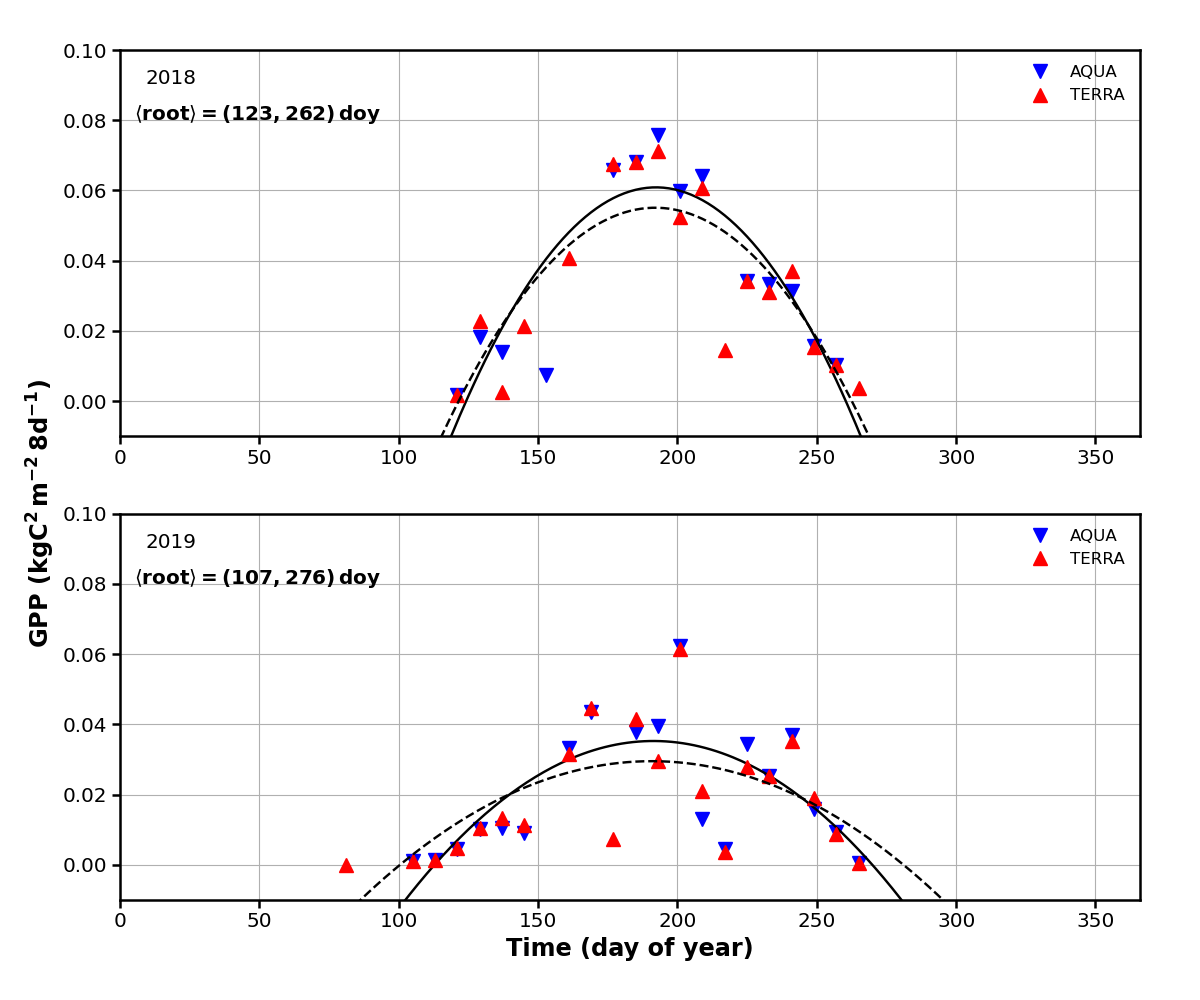
\includegraphics[width=0.75\textwidth]{./modis_Gpp.png}
    \caption{Estimated start and end of growing season from MODIS (Aqua/Terra) GPP over a $1\times 1$\,km patch centered at Svanhovd. The average start in 2018 amounts to doy 123 and to 107 in 2019. The end of the growing season in 2018 is doy 262 and in 2019 276.}
    \label{fig:modis_gpp}
\end{figure}

\item {\color{blue}Line 354. "A sample of downy birch leaves collected at Svanhovd had an average length of (3.0±0.5)cm" Were top-canopy leaves sampled? How many leaves were collected to get +- 0.5 cm standard error?}
Ane?

\item {\color{blue}Line 355. "We used 13.5m height"
Why was this value chosen? What is the meaning of a height between the average tree
height and the maximum tree heigh? Perhaps it would have been more reasonable to use
the average height.}
We suppose, the referee refers to the 10.1\,m average height of one particular Scots pine forest which has been measured in 2004. We assumed that after 14 year 10.1\,m might not be the average height of this particular forest anymore. In the absence of more recent measurements, we found it more reasonable to choose 13.5\,m the average tree height in the whole area in 2004 which included all tree species and ages.
We will include this in the text.

\item {\color{blue}Line 360 and following. POD1 was calculated by gap filling the data, right? Because there is a lot of data missing in the middle of the season. Or were POD1 compensated for missing data? If so, how? Please confirm it by writing it in the text.}
In Appendix~B2, we write that the "$\mathrm{DO_3SE}$ model requires hourly, continuous meteorologische observations." This means that all input data, including ozone, have to be gap filled before POD1 can be computed. The gap filling method for all data but ozone are described in appendix~B2. The used gap filling method for ozone has been summarized above (response to "Lines 206--208") and published in Falk et al. (2021). We shall restructure the text to make the description of the $\mathrm{DO_3SE}$ model and its input data clearer.

\item {\color{blue}Line 369. "Due to the shape of flight, a symmetric variation".
Symmetric variation of what?}
This refers to the variation of PPFD at a stomatal opening of 50\% by $\pm 20\%$ and the resulting response in computed POD1. We will make this clearer in the text.

\item {\color{blue}Line 370. "We find that an opening of stomata at lower light intensities can cause higher sensitivity to drought conditions." Please, explain where we can see this. Graph 8 is not clear at all to me. And then, "sensitivity" of what? Of plants? Of POD1?}
Figure~8 is indeed very complex and we will elaborate on the explanation and interpretation in the text to make it more accessible to the readers. You are right that this sentence is not clear and does not communicate what we intended to say. We refer to the sensitivity of modeled POD1. If we take a look at, e.g. Fig.~8a subarctic parameterazation and 2018 (left hand side of the upper panel). Open symbols represent a model simulation where SWP was taken into account. Closed symbols where this effect was switched off. The '--' symbolizes PPFD0.8 (earlier opening), the '+' PPFD1.2 (later opening). We shall have a look at the circles connected by a solide line representing the simulations with a GS which we have determined from temperatures. If the stomata open earlier / close later more ozone can be taken up (longer opening time), hence POD1 is larger than for the unchanged $f_\mathrm{light}$. Now, if we take SWP into account, we find that only the PPFD0.8 is affected. Therefore, we conclude that conditions that negatively affect SWP (referred to as droughts) reduce the uptake of ozone (POD1) when an earlier opening / later closing of stomata is considered. Hence, POD1 is more sensitive to drought conditions.

\item {\color{blue}Line 373. "The magnitude of these effects varies between PFTs as well as years, but the predicted ozone uptake for the bespoke temperature parameterization is always larger than for the MM parameterizations and of the same order of magnitude as the variability between the years studied here."
What effects? "Of the same order of magnitude as the interannual variability...": can you conclude it by comparing only two years? The same for line 402}
In Section~3, we tried to show that 2019 is representative for a normal year while 2018 is more extreme. We should evaluate our data with this question in mind and confirm that the difference between 2018 and 2019 is indeed representative for the interannual variability. Depending on the outcome, we will rephrase the sentences and substitute the term "interannual variability".

\item {\color{blue}Table 4.  Have the percentage of reduction been calculated taking into account pre-industrial concentrations as prescribed by the MM?
What are meaning of the superscripts? And, above all, why some superscripts indicate a range (e.g. 1.9 ... 2.1)? I did not understand how the stdev of the MM estimation was calculated, sorry.}
We will make this clearer in the next version of the manuscript. We used the relationship between biomass reduction and POD1 unchanged from the MM. This, however, is to some degree questionable because subarctic vegetation could be affected more or less by the same ozone dose than the central European species. Apparently, the caption of the table is not complete and parts of the explanation missing. We explain how we derive the uncertainty ranges in L405--407 but this may not be clear enough. From Fig.~8, we deduced that SWP is negligible in most cases (solid and open symbols show the same POD1). Hence, we computed the biomass reduction based on simulations with SWP effects on POD1 turned off and MM $f_\mathrm{light}$. The uncertainties reported are actually the differences and not standard deviations. The differences are calculated between the simulation with MM $f_\mathrm{light}$ and "bespoke" GS and the simulations with PPFD0.8 (larger POD1 $\rightarrow$ larger biomass reduction) and PPFD1.2 (smaller POD1 $\rightarrow$ less biomass reduction). The sub- and superscripts show the asymmetry introduced by the different $f_\mathrm{light}$ parameterizations. The range represents the additional uncertainty from the choice in GS.

\item {\color{blue}Line 416. "we have developed bespoke parameterizations"
it seems a bit strong statement to me, you have not developed any new tailored
parameterization, you have only hypothesized one. There is no one experiment nor
comparison with experimental results in your work.}
We will substitute the term to appropriately reflect our intensions and work.

\item {\color{blue}Line 417. "The comparison between meteorological conditions in 2018 and 2019 and their divergence from climatology allowed us to assess the influence of key environmental variables such as temperature, PPFD, and precipitation on vegetation susceptibility to O3 damage in light of future changes as may occur under climate change" I did not understand where all this "divergence with the climatological average" of these two years alone lies, sorry.}
We will make this clearer in the revision of the manuscript.

\item {\color{blue}Line 432. "With respect to ongoing climate change, a clear positive trend emerged in length (5.2d decade-1) of the growing season that is almost equally distributed between earlier start (2.9 days decade-1) and later end (2.3d decade-1) (Appendix Fig. A1)." How did you figure it out? Have you been doing retrospective MODIS analysis for 30 years? Or do you have a publication to quote?}
We have derived the number from an analysis of the thermal start and end of the GS based on the gridded temperature data from SeNorge.no provided by the Norwegian weather service and shown in Appendix Fig.~9. We may remove this part eventually or rephrase the sentence to include this information, support it with citations of relevant works, and include this analysis in a methods section.

\item {\color{blue}Line 435 and following. "visible damage"
Visible damage and POD can be totally unrelated, as demonstrated by some research
conducted on agricultural species. I recommend caution in stating that the O3 peaks
causing the visible symptoms can result in a biomass reduction (damage).}
You are absolutely right. We intended to state that visible damage and biomass reduction are not necessarily related in this paragraph. We agree that this is not clear and we will improve on this.

\item {\color{blue}Line 441. Does "damage" mean "visible leaf symptoms"? Or does it mean biomass reduction?}
See above. We will carefully rephrase the text with respect to the term "damage" and clearly distinguish between visible damage and biomass reduction.

\item {\color{blue}Line 456. "We found that soil water potential under 2018/19 meteorological conditions was negligible" What does it mean? That there was no water in the soil (SWP were negligible) or that the effect on the POD of the presence or absence of SWP in the calculation was negligible? Please clarify.}
The latter is correct. Thank you for pointing out this ambiguity.

\item {\color{blue}Line 461. "better suited" Point 1 is questionable.
Also point 2 is questionable. How can you say that the MM parameterization does not
capture the plant physiology of subactic vegetation if no comparisons with physiological measurements taken on subarctic vegetation are presented?}
We will adresse this point by reframing the storyline of the manuscript towards a new method to derive stomatal conductance parameterizations based on climatological and remotely sensed data. 

\item {\color{blue}Line 469. "However, the decline of this ozone spring peak is partly caused by the uptake of vegetation" Are you sure? Please cite a reference.}
We will rephrase this sentence to "[...] could partly be caused [...]". And may give a recap of ozone removal, as follows:
\emph{ozone is removed from the atmosphere by dry deposition which is described as a network of resistances. In general, snow and ice surfaces are found to have a low resistance to ozone , hence less ozone can be taken up by the land surface which is a major sink in absence of photochemical reactions (winter). Therefore, existing ozone accumulates in the subarctic winter boundary layer. The same goes for non-biogenic precursors. In spring these are chemically reactivated and increase the ozone production. At the same time coniferous trees might also start to produce BVOCs. At the same time, most of the vegetation is still covered by snow and ice and dry deposition remains low. In addition to the intrusion of stratospheric ozone, this causes the enhancement of ozone at the surface (spring peak). Now, with snowmelt and bud burst in spring, ozone dry deposition increases. Simultaneously, photochemical destruction of ozone also increases. Only part of ozone actually enters the stomata.}

\item {\color{blue}Line 491. "Automation of the here proposed PDF-based acclimation using machine learning techniques could overcome these issues in the future"
What does it mean? Please explain. Make an example.}
The proposed method to use climate data for adjusting the parameterization of stomatal conductance can be formulated as optimization problem (maximizing the enclosed temperature PDF area) which would make it possible to derive new parameters in an more automized way. 
Now, considering enough stomatal conductance data were available from observation in well known climate conditions these data could be used to evaluate our method and train a model to find the optimal stomatal conductance parameterization based on climate data alone. As climate data is more readily available compared to actual measurement of stomatal conductance this could help to improve modeling of stomatal conductance globally.

\item {\color{blue}Figure A1. How was the length of the growing seasons in the various years identified? By satellite? Other method? What does the gray band represent?} See response to "Line~432". The gray band represents the standard deviation. We will either remove or elaborate on this analysis.

\item {\color{blue}Line 511. "with fmin, Dmin, Dmax describing the relative stomatal conductance to changes in vapor pressure deficit." It is not clear. Please, clarify what D and fmin are, and their units.}

\item {\color{blue}
\begin{itemize}
    \item Line 517. "The DO3SE model as described in Büker et al. (2012) is used to simulate SWP0 across a PFT specific root depth according to the Penman--Monteith energy balance method that drives water cycling through the soil--plant--atmosphere system" I cannot understand how the P-M energy balance is used in DO3SE to derive the SWP. Please explain in detail.
    {\color{black} This is described in Bücker et al (2012) in detail. We will include an improved, short description of how the $\mathrm{DO_3SE}$ model incorporates the PM model to estimate evapotranspiration and hence water loss from the soil. However, for full details of this method it is best for readers to refer to Bücker et al. (2012).}

    \item Line 525.  "the concentration at the upper surface of the laminar layer for a sunlit upper canopy leaf" At what height was the O3 concentration measured? If it was not measured at the top of the canopy (10m for trees or 10 cm for grassland), how was the O3 concentration at the top canopy calculated? Please explain in detail.
    {\color{black} The $\mathrm{DO_3SE}$ model was used to estimate the difference in $[\mathrm{O_3}]$} between a reference height above the canopy and the canopy height. This employs the deposition component of the $\mathrm{DO_3SE}$ model that estimates the transfer of mass (i.e. ozone) as a function of windspeed, convection, surface roughness, and vegetation $[\mathrm{O_3}]$ sink. We will add additional detail in the paper to make this clear.

    \item Line 526.  What does rc represent? Is it the cuticular resistance or the bulk canopy resistance? What is its value?
    {\color{black}This represents cuticular resistance - we will include its value in the revision of the paper.}

    \item Line 528.  Can you explain where that formula for calculating the flux comes from? Why is there u(z1) in? And what is the z1 height?
    {\color{black}This comes from the $\mathrm{DO_3SE}$ model - we will add a suitable reference.}

    \item Line 531. What is the z1 height? Where is it?
    {\color{black}See above.}

    \item Line 535. Wind speed at 2 m: what is it used for? Please explain
    {\color{black}See above.}

    \item Section B1. The description of fPHEN is missing. Please, provide it. Again, how do you calculate the day-to-day SWP on your site? Please describe it in detail.
    {\color{black}See above.}
    
\end{itemize} }
We will make the description of the $\mathrm{DO_3SE}$ model more comprehensible and comprehensive. However, in the interest of the main focus of this manuscript it may not be possible to give a full recap of all details concerning this well established model.

\item {\color{blue}Line 550. Please explicitly describe the method used to gap-fill O3 concentrations because it could be crucial.}
See response to "Lines 206--208" above.


\item {\color{blue}Line 554. "From Fig. B1f) it is apparent that the mapping manual parameterized grassland would not have been able to grow in 2019." 
It does not seem to me that gstom has been reseted at all. If this is the case, the premises of the work appear weak.}
We indeed have no observational data to validate the suggested method at tis point.

\end{itemize}

\end{document}